\documentclass{article}

\usepackage[utf8]{inputenc}
\usepackage[brazilian]{babel}
\usepackage{graphicx}
\usepackage{float}
\usepackage[pdftex]{hyperref}
\usepackage{epstopdf}
\usepackage{etoolbox}
\usepackage{amsmath}
\usepackage{amsfonts}
\usepackage{amssymb}
\usepackage{caption}
\usepackage{subcaption}
\usepackage{setspace}
\usepackage{tikz}

\patchcmd{\thebibliography}{\section*}{\section}{}{}
\newcommand{\R}{\ensuremath{\mathbb{R}}}
\newcommand{\Prob}{\ensuremath{\mathbb{P}}}
\newcommand{\K}{\ensuremath{\mathbb{K}}}
\newcommand{\U}{\ensuremath{\mathbb{U}}}
\newcommand{\N}{\ensuremath{\mathbb{N}}}
\newcommand{\Lg}{\ensuremath{\mathbb{L}}}
\newcommand{\T}{\ensuremath{\rm Tr}}
\newcommand{\sg}{{\sigma(x_k)}}

\newcommand{\G}{\ensuremath{\mathcal{G}}}
\newcommand{\F}{\ensuremath{\mathcal{F}}}
\newcommand{\C}{\ensuremath{\mathcal{C}}}
\newcommand{\E}{\ensuremath{\mathcal{E}}}
\newcommand{\Hn}{\ensuremath{\mathcal{H}}}
%\newcommand{\Hoo}{\ensuremath{\mathcal{H}_\infty}}
\newcommand{\Hop}{\ensuremath{\mathcal{H}_{op}}}
% --------------------------------------------------
\newtheorem{theo}{Teorema}
\newtheorem{exa}{Exemplo}
\newtheorem{lemm}{Lema}
\newtheorem{coro}{Corolário}
\newtheorem{defn}{Definição}[section]

%opening


\begin{document}
\input{capa.tex}

\onehalfspacing
\section{Objetivos} 
O objetivo desse experimento foi o projeto e análise de um controlador via realização em espaço de estado e um observador de estado para a planta eletrônica identificada no experimento 2\cite{bb:lab2}. 
	
\section{Projeto do Controlador}
Como nossa planta apresentou problemas durante o decorrer do experimento, apresentando respostas diferentes para o mesmo controlador de acordo com a temperatura do circuito e a posição em que esta se encontrava (provavelmente devido a componentes defeituosos e mal contatos), nós, conforme sugerido pela professora, refizemos o experimento utilizando a planta número 8.
Essa planta teve sua função de transferência, representada pela equação \ref{eq:gs}, calculada por outro grupo usando as medidas realizadas durante o experimento 2 e nós, através do seu relatório\cite{bb:lab2gui}, recuperamos esses valores e utilizamos a mesma metodologia utilizada no pré relatório \cite{bb:prelab6} para o projeto do controlador e observador em espaço de estado conforme a figura \ref{fig:contrss}, com as matrizes $A$, $B$ e $C$ indicadas em \ref{eq:mata}, \ref{eq:matb} e \ref{eq:matc}.\\

\begin{equation}
\label{eq:gs}
G(s) = \frac{\kappa_1\kappa_2\kappa_3\kappa_4}{(s\tau_2 + 1)(s\tau_3 + 1)s}
\end{equation}

\begin{table}[H]
	\centering
	\caption{Parâmetros numéricos da função de transferência}
	\label{tab:valores}
	\begin{tabular}{|c|c|}
		\hline Parâmetro & Valor \\ 
		\hline $\kappa_1$ & $-0.0995$\\ 
		\hline $\kappa_2$ & $-2.1626$\\ 
		\hline $\kappa_3$ & $-4.5739$\\ 
		\hline $\kappa_4$ & $-9.1333$\\ 
		\hline $\tau_2$ & $0.0130$\\ 
		\hline $\tau_3$ & $0.0232$ \\ 	
		\hline 
	\end{tabular} 
\end{table}

\begin{figure}[H]
	\centering
	\includegraphics[width=0.8\linewidth]{contrss}
	\caption{Diagrama de blocos do sistema}
	\label{fig:contrss}
\end{figure}

\begin{equation}
\label{eq:mata}
A=
\begin{bmatrix}
 0 & 1 & 0 \\
 0 & 0 & 1 \\
 0 & -\frac{1}{\tau_2\tau_3} & -\frac{\tau_2+\tau_3}{\tau_2\tau_3}
\end{bmatrix}
\end{equation}
\begin{equation}
\label{eq:matb}
B=
\begin{bmatrix}
0 \\
0 \\
\frac{\kappa_1\kappa_2\kappa_3\kappa_4}{\tau_2\tau_3}
\end{bmatrix}
\end{equation}
\begin{equation}
\label{eq:matc}
C=
\begin{bmatrix}
1 & 0 & 0
\end{bmatrix}
\end{equation}

Através dessas matrizes e das especificações do projeto determinamos as matrizes K, L e M para a implementação do sistema conforme detalhado no pré roteiro, porém alteramos os autovalores desejados para o observador de maneira a aumentar sua velocidade de resposta. Definimos que esses novos autovalores deveriam ser da ordem de 5 vezes maiores que o maior autovalor do controlador, logo escolhemos 
\subsection{Requisitos do Sistema e Projeto}
Seguindo o proposto no roteiro \cite{bb:roteiro} as especificações do sistema são:
\begin{itemize}
	\item Tempo de estabilização de aproximadamente $0.5$ [s].
	\item Fator de amortecimento igual a $\sqrt{2}/2$.
	\item Polo em $s=-30$.
	\item Erro em regime permanente nulo a uma entrada rampa.
	\item Amplitude do sinal de controle não pode ultrapassar $\pm10$ [Volts].
\end{itemize}\

\subsection{Calculo de K}
Considerando que o tempo de estabilização do sistema é influenciado principalmente pelos dois polos de menor parte real, podemos aproximar o sistema como de segunda ordem e calcular os polos que cumprem os dois primeiros requisitos. Escolhemos então o terceiro polo do sistema conforme especificado, obtendo:
\begin{equation}
	s_1=-7.8240 + 7.8240i
\end{equation}
\begin{equation}
	s_2=-7.8240 - 7.8240i
\end{equation}
\begin{equation}
	s_3=-30
\end{equation}

Utilizando a metodologia indicada no roteiro\cite{bb:roteiro}, encontramos K que aloca os autovalores da matriz $A - BK$ nos polos desejados, chegamos então a: 
\begin{equation}
\label{eq:matk}
K=
\begin{bmatrix}
0.3329 & -0.1232 & -0.0039
\end{bmatrix}
\end{equation}

\subsection{Calculo de L}
A matriz L nos permite alocar os polos de nosso observador. Desejamos que este siga o estado do sistema de maneira mais rápida possível, ou seja, tenha um tempo de resposta menor que o controlador, porém sem que sua largura de faixa seja muito larga (para diminuir a influência de ruídos). Escolhemos então como polos do observador o dobro dos polos do controlador, obtendo L que aloca os polos da matriz $A - LC$ conforme o desejado:
\begin{equation}
\label{eq:matl}
L=
\begin{bmatrix}
2.6935 & 177.2424 & 8422.7
\end{bmatrix}
\end{equation}

\subsection{Calculo de M}
Para cumprir a quarta especificação, devemos encontrar a matriz M que satisfaz as equações \ref{eq:m1} e \ref{eq:m2}.
\begin{equation}
\label{eq:m1}
S(0)KM(0) = 1
\end{equation}
\begin{equation}
\label{eq:m2}
(\frac{d}{ds}(S(s)KM(s)))_{s=0}= 0
\end{equation}
Conforme sugerido no roteiro\cite{bb:roteiro}, escolhemos M da forma:
\begin{equation}
\label{eq:mlayout}
M = \frac{\frac{s}{\tau} + 1}{\frac{s}{30} + 1}\begin{bmatrix}
m_1\\
m_2\\
m_3
\end{bmatrix}
\end{equation}
Obtivemos então as equações:
\begin{equation}
	m_1 - 0.3702m_2 - 0.0117m_3 = 1
\end{equation}
\begin{equation}
	\frac{1}{\tau} - 0.1945 = 0
\end{equation}
Como os valores de $m_1$, $m_2$ e $m_3$ pouco afetam a resposta do sistema, desde que sigam as equações acima, escolhemos arbitrariamente os valores $m_1 = 1$ e $m_2 = 0.5$ e resolvemos o sistema, obtendo:
\begin{equation}
\label{eq:mvalor}
M = \frac{\frac{s}{5.142} + 1}{\frac{s}{30} + 1}*
\begin{bmatrix}
	1\\
	0.5\\
	-15.8275
\end{bmatrix}
\end{equation}

\subsection{Implementação}
Para realizar o sistema, seguimos a estrutura recomendada no roteiro\cite{bb:roteiro}, obtendo a implementação mostrada na figura \ref{fig:impl} com as funções de transferência \ref{eq:hs}, \ref{eq:cus} e \ref{eq:cys}.
\begin{figure}[H]
	\centering
	\includegraphics[width=0.8\linewidth]{impl}
	\caption{Diagrama de blocos da implementação final do controle}
	\label{fig:impl}
\end{figure}

\begin{equation}
\label{eq:hs}
h(s) = KM(s) = \frac{1.942s+9.987}{s+30}
\end{equation}
\begin{equation}
\label{eq:cus}
C_u(s) = K(sI - (A - LC))^{-1}B = \frac{-42.95s^2-1475s-7603}{s^3+91.3s^2+2367s+29380}
\end{equation}
\begin{equation}
\label{eq:cys}
C_y(s) = K(sI - (A - LC))^{-1}L = \frac{-53.74s^2-1488s+9782}{s^3+91.3s^2+2367s+29380}
\end{equation}


\section{Simulação}
Com o auxílio do Simulink simulamos (com e sem ruído branco) as respostas do controlador a uma onda quadrada de amplitude $1V$ e frequência de $0,25Hz$, e seus esforços de controle, que podem ser vistas nas figuras \ref{fig:yur} e \ref{fig:yurN}.
\begin{figure}[H]
	\centering
	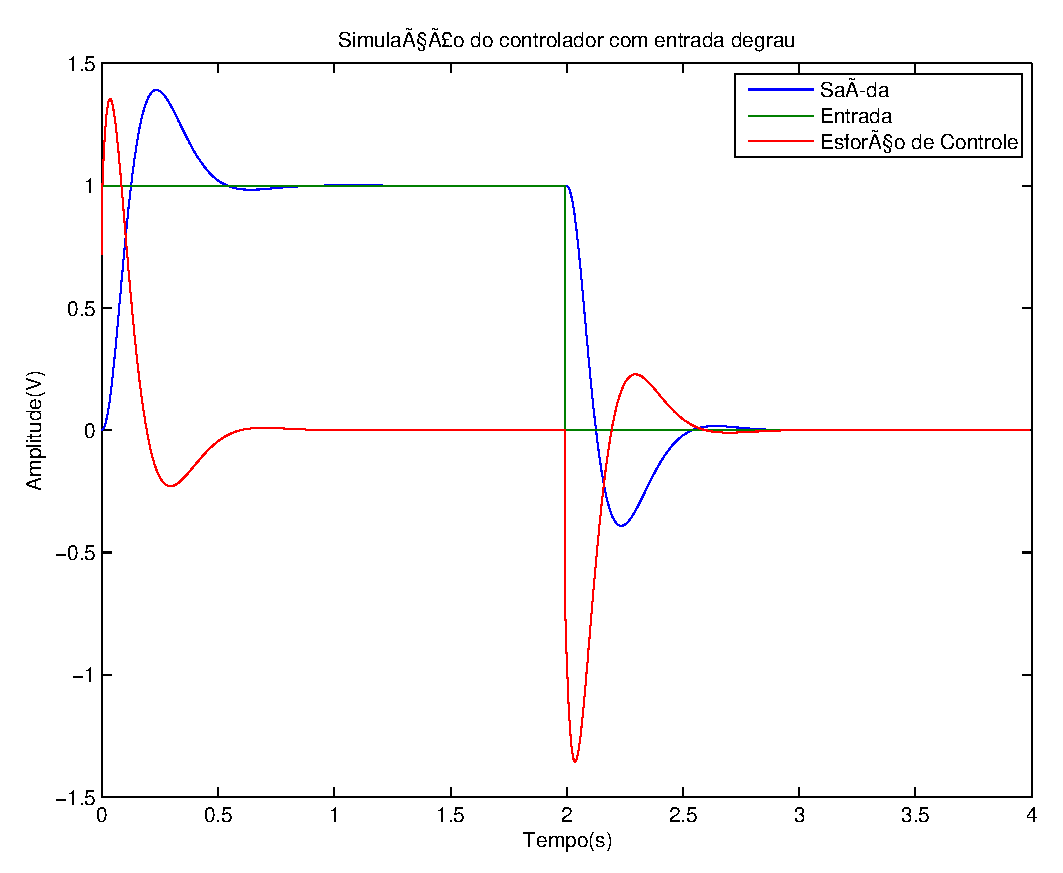
\includegraphics[width=0.8\linewidth]{../yur}
	\caption{Resposta e esforço de controle para onda quadrada}
	\label{fig:yur}
\end{figure}
\begin{figure}[H]
	\centering
	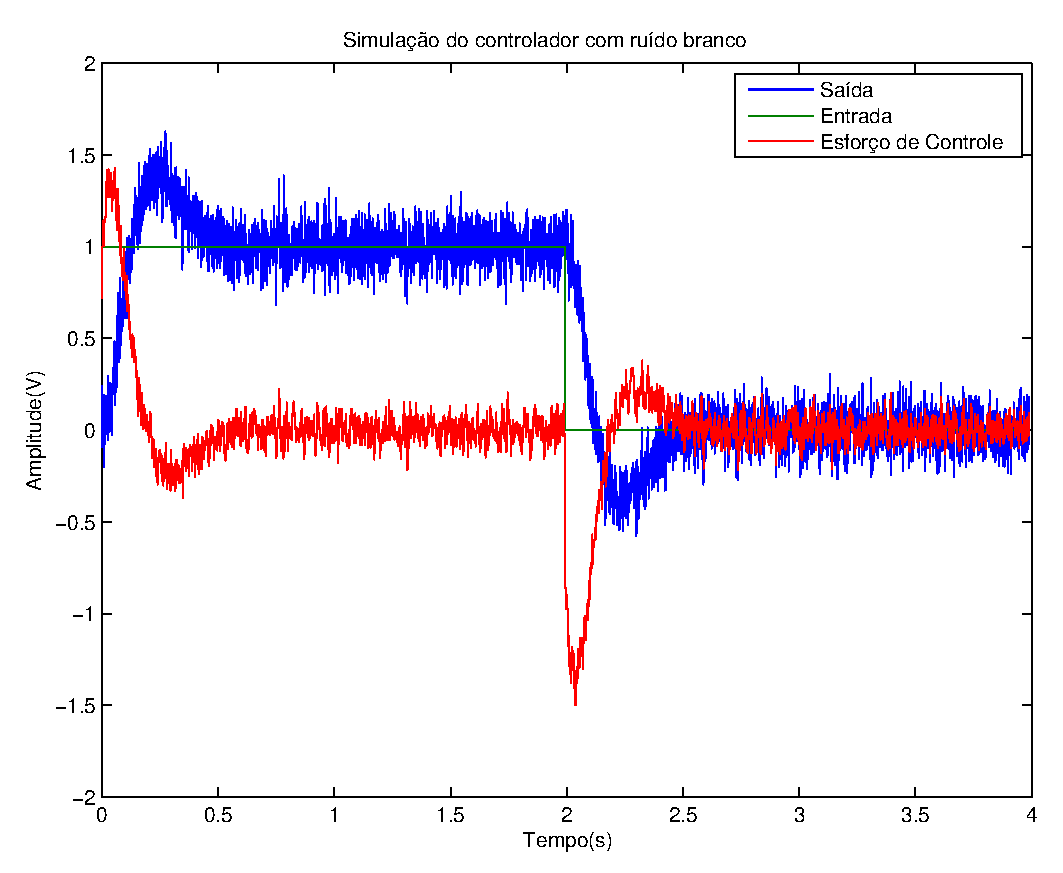
\includegraphics[width=0.8\linewidth]{../yurN}
	\caption{Resposta e esforço de controle para onda quadrada, com ruído branco}
	\label{fig:yurN}
\end{figure}

Para analisar a eficiência do nosso observador, simulamos o modelo no espaço de estados (em torno do ponto de equilíbrio [0,0,0]', com estado inicial do controlador [0, 0, 0]' e do observador [1, 0, 0]') e plotamos o estado do sistema e o estado estimado pelo observador, que podem ser vistos nas figuras \ref{fig:obsx1}, \ref{fig:obsx2} e \ref{fig:obsx3}.
\begin{figure}[H]
	\centering
	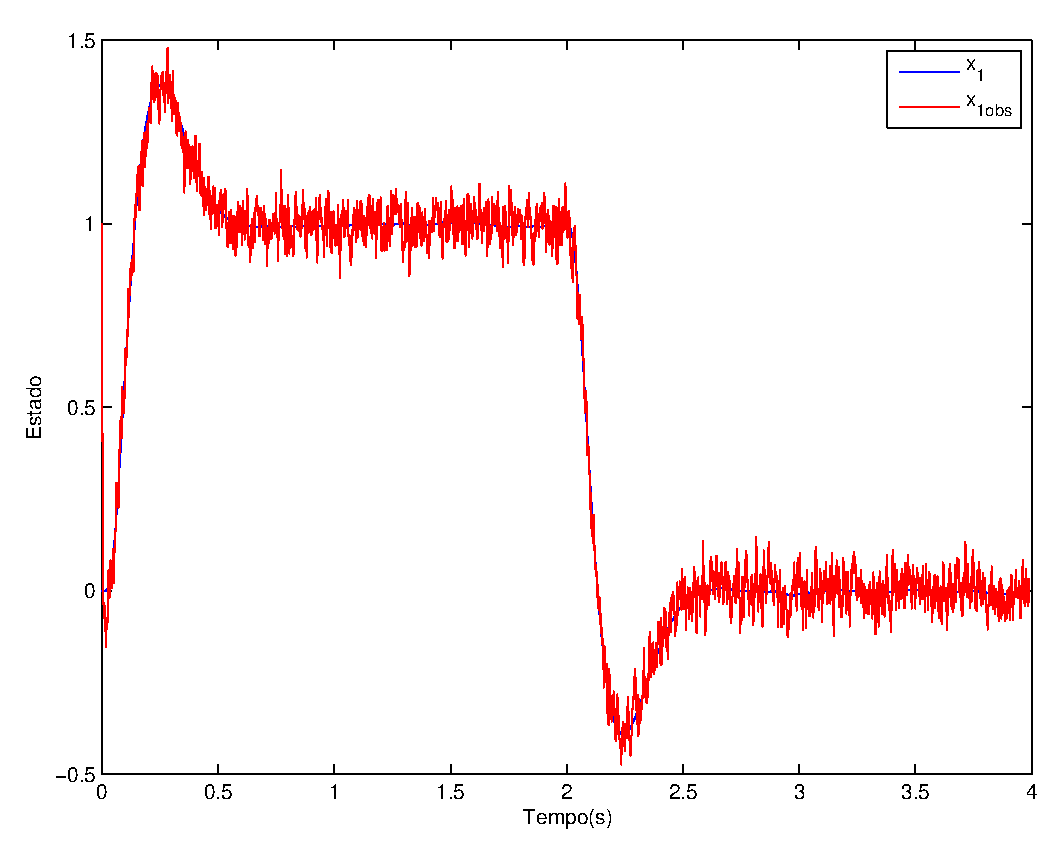
\includegraphics[width=0.8\linewidth]{../obsx1}
	\caption{Estado $x_1$ real e estimado do sistema para onda quadrada, com ruído branco}
	\label{fig:obsx1}
\end{figure}
\begin{figure}[H]
	\centering
	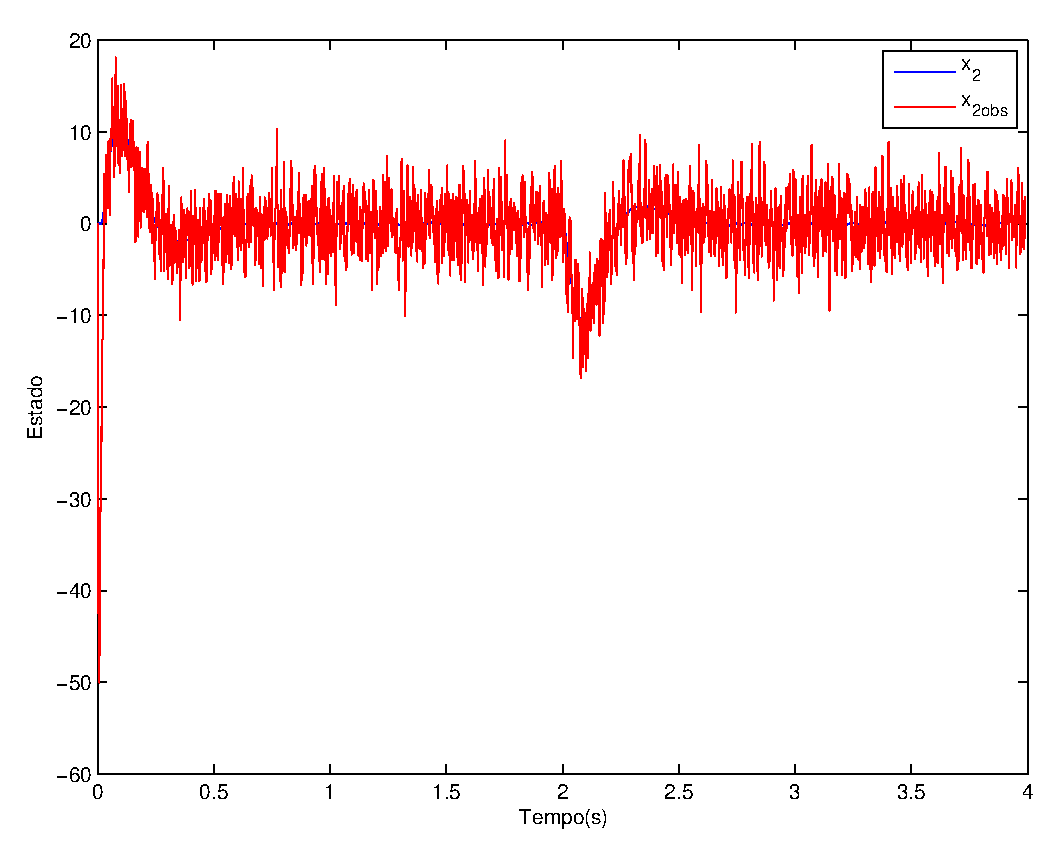
\includegraphics[width=0.8\linewidth]{../obsx2}
	\caption{Estado $x_2$ real e estimado do sistema para onda quadrada, com ruído branco}
	\label{fig:obsx2}
\end{figure}
\begin{figure}[H]
	\centering
	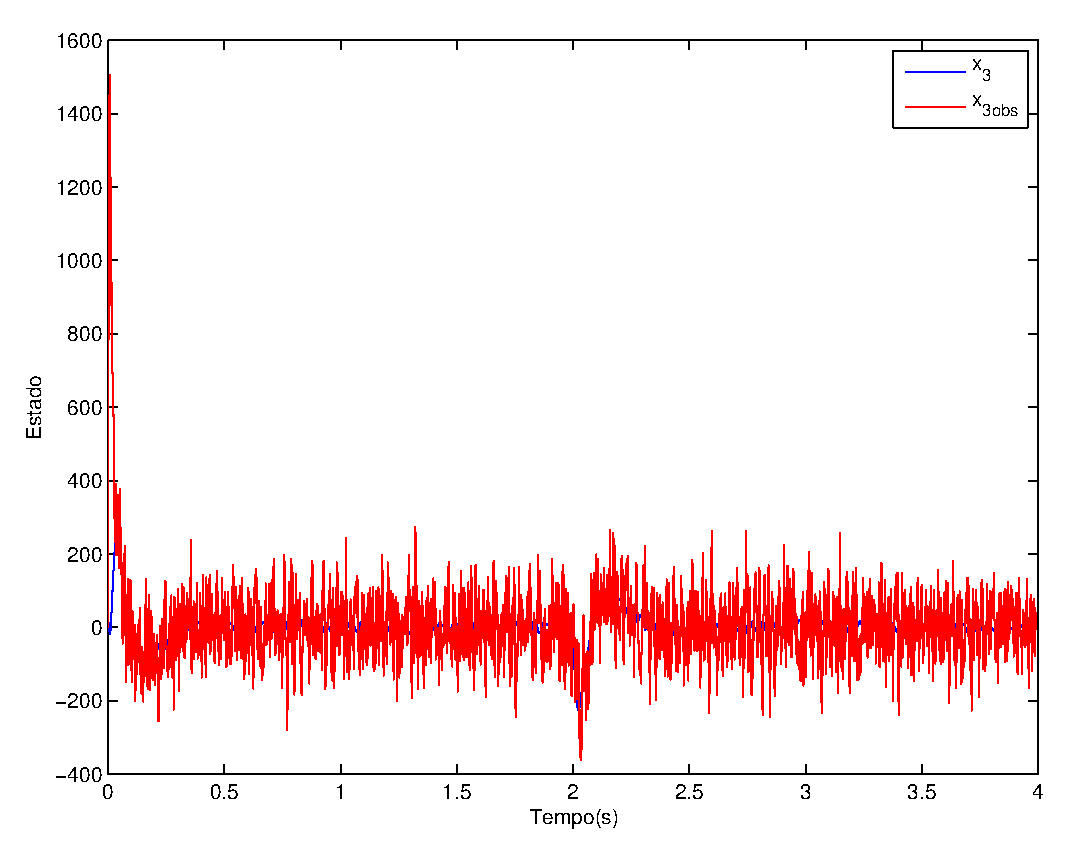
\includegraphics[width=0.8\linewidth]{../obsx3}
	\caption{Estado $x_3$ real e estimado do sistema para onda quadrada, com ruído branco}
	\label{fig:obsx3}
\end{figure}
Como podemos ver o observador projetado segue bem o sistema real e não foi gravemente afetado pelo ruído.


Simulamos também a resposta deste controlador a uma rampa, mostrada na figura \ref{fig:yurR}. Como podemos ver, o erro estacionário para essa entrada é nulo, conforme desejado.
\begin{figure}[H]
	\centering
	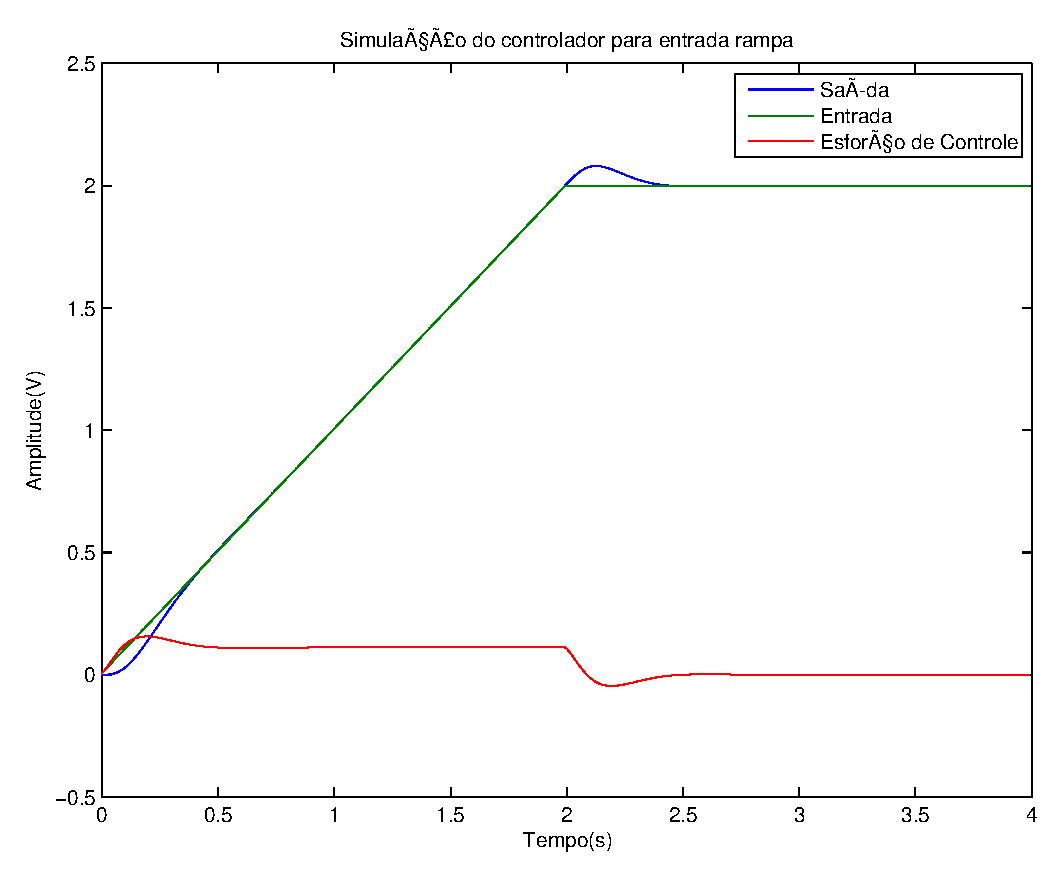
\includegraphics[width=0.8\linewidth]{../yurR}
	\caption{Resposta e esforço de controle para rampa}
	\label{fig:yurR}
\end{figure}
A tabela \ref{tab:stepinfo} apresenta as características da resposta desse controlador, obtida com o auxílio da função \textit{stepinfo} do Matlab.
\begin{table}[H]
	\centering
	\caption{Características da resposta do controlador}
	\label{tab:stepinfo}
	\begin{tabular}{|c|c|}
		\hline Sobrelevação 				& $39.1095\%$ \\ 
		\hline Tempo de estabilização 		& $0.5089$ [s]\\ 
		\hline Tempo de subida				& $0.0835$ [s]\\ 
		\hline Erro estacionário (degrau) 	& $0$\\ 
		\hline Erro estacionário (rampa) 	& $0$\\ 
		\hline 
	\end{tabular} 
\end{table}

Como podemos ver o sistema atinge todas as especificações e não é muito susceptível a ruídos, porém ele apresenta uma sobrelevação bastante significativa. Nossa análise mostra que essa sobrelevação está associada à matriz M, porque quando relaxamos o critério de erro estacionário à rampa observa-se uma diminuição do overshoot para $5\%$.


Isso acontece pois essa matriz acrescenta um zero (em $- 5.142$) no sistema. O efeito desse zero pode ser visto se levamos em consideração a função de transferência:
\begin{equation}
	H_z(s) = (\frac{s}{z} + 1)H(s) = H(s) + \frac{1}{z}sH(s)
\end{equation}
Logo a resposta ao degrau do sistema acrescentado de um zero será da forma:
\begin{equation}
Y_z(s) = (H(s) + \frac{1}{z}sH(s))\frac{1}{s} = H(s)\frac{1}{s} + \frac{s}{z}H(s)\frac{1}{s} = Y(s) + \frac{s}{z}Y(s)
\end{equation}
Tirando a transformada de Laplace inversa:
\begin{equation}
y_z(t) = y(t) + \frac{1}{z}\dot{y}(t)
\end{equation}
Podemos ver então que ao acrescentar um zero no sistema nós somamos um termo derivativo à resposta original, o que causa um aumento na sobrelevação e uma aceleração na resposta do sistema (uma vez que nas transições a derivada terá um valor significativo). Para anular o efeito desse zero nós precisaríamos aumentar seu valor absoluto, porém para fazer isso e ainda cumprir a exigência de erro estacionário nulo para à rampa precisaríamos alterar a matriz K, o que implicaria no não cumprimento das outras exigências do projeto.
\begin{thebibliography}{widestlabel}
	\bibitem{bb:roteiro}{Roteiro do experimento disponibilizado para os alunos}
	\bibitem{bb:lab2}{KIAN, Marcelli; OLIVEIRA, Daniel. \textit{Relatório - Experimento 2:} Identificação de plantas eletrônicas.}
\end{thebibliography}
\end{document}

